%!TEX program = xelatex
\documentclass[11pt,a4paper]{article}
\usepackage[utf8]{inputenc}
\usepackage[T1]{fontenc}
\usepackage{ctex}
\usepackage{authblk}
\usepackage{tikz}
\usepackage{pgfplots}
\usepackage{verbatim}
\usepackage{amsfonts}
\usepackage{amsmath}
\usepackage{amsthm}
\usepackage{indentfirst}
\usepackage{amssymb}
\setlength{\parindent}{0pt}
\usetikzlibrary{shapes,snakes}
\newcommand{\argmax}{\operatornamewithlimits{argmax}}
\newcommand{\argmin}{\operatornamewithlimits{argmin}}

\DeclareMathOperator{\col}{col}
\usepackage{booktabs}
\newtheorem{theorem}{Theorem}
\newtheorem{proposition}{Proposition}
\newtheorem{lemma}{Lemma}
\newtheorem{example}{Example}
\newtheorem{corollary}{Corollary}
\newtheorem{note}{Note}
\usepackage{graphicx}
\usepackage{geometry}
\usepackage{hyperref}
\newcommand{\code}{	exttt}
\geometry{a4paper,scale=0.8}
\title{Linear Algebra}
\author[*]{Wenxiao Yang}
\affil[*]{Department of Mathematics, University of Illinois at Urbana-Champaign}
\date{2021}





\begin{document}
\maketitle
\tableofcontents
\newpage

\section{Vector Space}
\subsection{Vector Space $(V,+,\times)$ (over a field $\mathbb{F}$)}
A \underline{vector space} over a field $\mathbb{F}$ is a
set $V$ w/ an operation \underline{addition} $+ : V \times V \rightarrow V$ and
an operation \underline{scalar multiplication} $\mathbb{F} \times V \rightarrow V$\\
(1) Addition is associative $\&$ commutative\\
(2) $\exists 0\in V$, additive identity: $0 + v = v \forall v \in V$\\
(3) $1v = v \forall v \in V$(where $1 \in \mathbb{F}$ is multi. id. in $\mathbb{F}$ )\\
(4) $\forall \alpha,\beta\in\mathbb{F},\ v\in V,\ \alpha(\beta v)=(\alpha\beta)v$\\
(5) $\forall v\in V,\ (-1)v=-v$ we have $v+(-v)=0$\\
(6) $\forall \alpha\in\mathbb{F},\ v,u\in V,\ \alpha(v+u)=\alpha v+\alpha u$\\
(7) $\forall \alpha,\beta\in\mathbb{F},\ v\in V,\ (\alpha+\beta)v=\alpha v+\beta v$

\subsection{A field is a vector space over its subfield}
\begin{example}
$\mathbb{K}\subset\mathbb{F}$ is a subfield of a field $\mathbb{F}$. Then $\mathbb{F}$ is a vector space over $\mathbb{K}$. (Since $\mathbb{F}\subset \mathbb{F}[x]$, then $\mathbb{F}[x]$ is a vector space over $\mathbb{F}$.)
\end{example}
\subsection{ Vector subspace}
Suppose that $V$ is a vector space over $\mathbb{F}$. A \underline{vector subspace} or just \underline{subspace} is a nonempty subset $W\subset V$ closed under addition and scalar multiplication. i.e. $v+w\in W,\ av\in W,\ \forall v,w\in W,\ a\in \mathbb{F}$.\\
\begin{example}
$\mathbb{K}\subset \mathbb{L}\subset \mathbb{F}$, then $\mathbb{L}$ is a subspace of $\mathbb{F}$ over $\mathbb{K}$.
\end{example}
\subsection{Linear independent, Linear combination}
\subsection{span V, basis, dimension}
A set of elements $v_1,...,v_n\in V$ is said to \textbf{span} $V$ if every vector $v\in V$ can be expressed as a linear combination of $v_1,...,v_n$. If $v_1,...,v_n$ spans and is linearly independent, then we call the set a \textbf{\textit{basis}} for $V$.
\begin{proposition}[Proposition 2.4.10.]
    Suppose $V$ is a vector space over a field $\mathbb{F}$ having a basis $\{v_1,...,v_n\}$ with $n \geq 1$.
\end{proposition}
(i) For all $v \in V$ , $v = a_1 v_1 + ... + a_n v_n$ for exactly one $(a_1,...,a_n)\in \mathbb{F}^n$.\\
(ii) If $w_1,...,w_n$ span $V$ , then they are linearly independent.\\
(iii)If $w_1,...,w_n$ are linearly independent, then they span $V$.\\
If a vector space $V$ over $\mathbb{F}$ has a basis with $n$ vectors, then $V$ is said to be n-dimensional (over $\mathbb{F}$) or is said to have \textbf{dimension} $n$.
\subsection{Standard basis vectors}
\begin{equation}
    \begin{aligned}
        e_1=(1,0,...,0),e_2=(0,1,0,...,0),...,e_n=(0,0,...,0,1)\in \mathbb{F}^n
    \end{aligned}
    \nonumber
\end{equation}
are a basis for $\mathbb{F}^n$ called the \textbf{standard basis vectors}.
\subsection{Linear transformation}
Given two vector spaces $V$ and $W$ over $\mathbb{F}$ a \textbf{linear transformation} is a function $T : V \rightarrow	 W$ such that
for all $a \in \mathbb{F}$ and $v,w \in V$ , we have
\begin{equation}
    \begin{aligned}
        T(av)=aT(v)\ and\ T(v+w)=T(v)+T(w)
    \end{aligned}
    \nonumber
\end{equation}
\begin{proposition}[Proposition 2.4.15.]
    If $V$ and $W$ are vector spaces and $v_1,...,v_n$ is a basis for $V$ then any function
    from $\{v_1,...,v_n\}\rightarrow W$ extends \textit{uniquely} to a linear transformation $V \rightarrow W$.
\end{proposition}
Any $v\in V$, $\exists (a_1,...,a_n)$ s.t. $v=a_1 v_1+...+a_n v_n$. Then $T(v)=T(a_1 v_1+...+a_n v_n)=a_1T(v_1)+...+a_nT(v_n)$\\
\subsection{一个线性变换对应一个矩阵, 线性变换矩阵相乘仍为线性变换矩阵}
\begin{corollary}[Corollary 2.4.16.]
    If $v_1,...,v_n$ is a basis for a vector space $V$ and $w_1,...,w_n$ is a basis for a vector space $W$ (both over $\mathbb{F}$), then any linear transformation $T : V \rightarrow W$ determines (and is determined by) the $m\times n$ matrix:
    \begin{equation}
        \begin{aligned}
            A=A(T)=\begin{bmatrix}
                A_{11}&	A_{12}&... &A_{1n}\\
                A_{21}&	A_{22}&... &A_{2n}\\
                \vdots&	\vdots&... &\vdots\\
                A_{m1}&	A_{m2}&... &A_{mn}
            \end{bmatrix}
        \end{aligned}
        \nonumber
    \end{equation}
\end{corollary}
\begin{equation}
    \begin{aligned}
        &\begin{bmatrix}
            w_1&\cdots	&w_m
        \end{bmatrix}^T=A
        &\begin{bmatrix}
                v_1&\cdots	&v_n
        \end{bmatrix}^T
    \end{aligned}
    \nonumber
\end{equation}
$\mathcal{L} (V,M)$ denotes the set of all linear transformations from $V$ to $W$; $M_{m\times n}(\mathbb{F})$ the set of $m\times n$ matrix with entries in $\mathbb{F}$. $T\rightarrow A(T)$ defines a \textit{bijection} $\mathcal{L} (V,M)\rightarrow M_{m\times n}(\mathbb{F})$. \textbf{$A(T)$ represents the linear transformation $T$}.


\begin{proposition}[Proposition 2.4.19]
    Suppose that $V$ , $W$, and $U$ are vector spaces over $\mathbb{F}$, with fixed chosen bases. If
    $T : V \rightarrow W$ and $S : W \rightarrow U$ are linear transformations represented by matrices $A = A(T)$ and $B = B(S)$,
    then $ST = S \circ T : V \rightarrow U$ is a linear transformation represented by the matrix $BA = B(S)A(T)$.
\end{proposition}

\subsection{GL(V): invertible linear transformations $V \rightarrow	V$}
Given a vector space $V$ over $F$, we let $GL(V ) \subset \mathcal{L}(V , V )$ denote the subset of \textbf{invertible linear transformations}.
\begin{equation}
    \begin{aligned}
        GL(V)=\{T\in \mathcal{L}(V , V )| T \textit{ is a bijection}\}=\mathcal{L}(V , V )\cap Sym(V)
    \end{aligned}
    \nonumber
\end{equation}

\section{Eigenvalues Related}
\subsection{Eigenvalues, Eigenvectors}
\subsubsection{Definition}
A vector $x$ is an $\textbf{eigenvector}$ of a matrix $A$ if $Ax$ is parallel to $x$, that is if $Ax = \lambda x$ for some number $\lambda\in \mathbb{R}$. The number $\lambda$ is called an $\textbf{eigenvalue}$ of $A$.

i.e. the root of $(A-\lambda I_n)x=0 \Leftrightarrow det(A-\lambda I_n)=0$

\subsubsection{Diagonalizable Matrix}
A $n\times n$ matrix $A$ with $n$ linearly independent eigenvalues $u$ is said to be diagonalizable.
\begin{equation}
    \begin{aligned}
        AU&=A\begin{bmatrix}
            |&|&\cdots&|\\
            u_1&u_2&\cdots&u_n\\
            |&|&\cdots&|
        \end{bmatrix}\\
        &=\begin{bmatrix}
            |&|&\cdots&|\\
            \lambda_1u_1&\lambda_2u_2&\cdots&\lambda_nu_n\\
            |&|&\cdots&|
        \end{bmatrix}\\
        &=\begin{bmatrix}
            |&|&\cdots&|\\
            u_1&u_2&\cdots&u_n\\
            |&|&\cdots&|
        \end{bmatrix}\begin{bmatrix}
            \lambda_1&&&\\
            &\lambda_2&&\\
            &&\ddots&\\
            &&&\lambda_n
        \end{bmatrix}\\
        &=UD\\
        \Rightarrow	A=UDU^{-1}
    \end{aligned}
    \nonumber
\end{equation}

\begin{theorem}
    If an $n\times n$ matrix $A$ has $n$ linearly independent eigenvectors $u_1,...,u_n$ corresponding to eigenvalues $\lambda_1,...,\lambda_n$, then $A = UDU^{−1}$ where $D$ is diagonal with entries $\lambda_1,...,\lambda_n$, and $U$ has columns $u_1,...,u_n$.
\end{theorem}

\subsection{Jacobian matrix}
Suppose $\mathbf{f}: \mathbf{R}^{n} \rightarrow \mathbf{R}^{m}$ is a function such that each of its first-order partial derivatives exist on $\mathbf{R}^{n} .$ This function takes a point $\mathbf{x} \in \mathbf{R}^{n}$ as input and produces the vector $\mathbf{f}(\mathbf{x}) \in \mathbf{R}^{m}$ as output. Then the Jacobian matrix of $\mathbf{f}$ is defined to be an $m \times n$ matrix, denoted by $\mathbf{J}$, whose $(i, j)$ th entry is $\mathbf{J}_{i j}=\frac{\partial f_{i}}{\partial x_{j}}$, or explicitly

$
\mathbf{J}=\left[\begin{array}{ccc}
\frac{\partial \mathbf{f}}{\partial x_{1}} & \cdots & \frac{\partial \mathbf{f}}{\partial x_{n}}
\end{array}\right]=\left[\begin{array}{c}
\nabla^{\mathrm{T}} f_{1} \\
\vdots \\
\nabla^{\mathrm{T}} f_{m}
\end{array}\right]=\left[\begin{array}{ccc}
\frac{\partial f_{1}}{\partial x_{1}} & \cdots & \frac{\partial f_{1}}{\partial x_{n}} \\
\vdots & \ddots & \vdots \\
\frac{\partial f_{m}}{\partial x_{1}} & \cdots & \frac{\partial f_{m}}{\partial x_{n}}
\end{array}\right]
$

where $\nabla^{\mathrm{T}} f_{i}$ is the transpose (row vector) of the gradient of the $i$ component.

\subsection{Hessian matrix}
Suppose $f: \mathbb{R}^{n} \rightarrow \mathbb{R}$ is a function taking as input a vector $\mathbf{x} \in \mathbb{R}^{n}$ and outputting a scalar $f(\mathbf{x}) \in \mathbb{R}$. If all second partial derivatives of $f$ exist and are continuous over the domain of the function, then the Hessian matrix $\mathbf{H}$ of $f$ is a square $n \times n$ matrix, usually defined and arranged as follows:

$
\mathbf{H}_{f}=\left[\begin{array}{cccc}
\frac{\partial^{2} f}{\partial x_{1}^{2}} & \frac{\partial^{2} f}{\partial x_{1} \partial x_{2}} & \cdots & \frac{\partial^{2} f}{\partial x_{1} \partial x_{n}} \\
\frac{\partial^{2} f}{\partial x_{2} \partial x_{1}} & \frac{\partial^{2} f}{\partial x_{2}^{2}} & \cdots & \frac{\partial^{2} f}{\partial x_{2} \partial x_{n}} \\
\vdots & \vdots & \ddots & \vdots \\
\frac{\partial^{2} f}{\partial x_{n} \partial x_{1}} & \frac{\partial^{2} f}{\partial x_{n} \partial x_{2}} & \cdots & \frac{\partial^{2} f}{\partial x_{n}^{2}}
\end{array}\right],
$

or, by stating an equation for the coefficients using indices $i$ and $j$,

$
\left(\mathbf{H}_{f}\right)_{i, j}=\frac{\partial^{2} f}{\partial x_{i} \partial x_{j}} .
$

The Hessian matrix is a symmetric matrix, since the hypothesis of continuity of the second derivatives implies that the order of differentiation does not matter (Schwarz's theorem).

The determinant of the Hessian matrix is called the Hessian determinant.

\subsection{Positive Definite Matrices}
\subsubsection{Definition}
We say that a symmetric $n \times n$ matrix $A$ is:

(1). $\textbf{ positive semidefinite}$ (written $A \succeq 0$) if $x^TAx \geq 0$ for all $x$.

(2). $\textbf{ positive definite}$ (written $A \succ 0$) if $x^TAx > 0$ for all $x\neq 0$.

(3). $\textbf{ negative semidefinite}$ (written $A \preceq 0$) if $x^TAx \leq 0$ for all $x$.

(4). $\textbf{ negative definite}$ (written $A \prec 0$) if $x^TAx < 0$ for all $x\neq 0$.

(5). $\textbf{ indefinite}$ (not written in any particular way) if none of the above apply.

$x^TAx$ is a function of $x$ called the quadratic form associated to $A$.

$\textbf{Note:}$ $A^TA$ is $\textbf{ positive semidefinite}$, since $x^TA^TAx=\|Ax\|^2\geq 0$.

\subsubsection{Diagonal matrix situation}
$$D=\begin{bmatrix}
    d_1&0&... &0\\0&d_2&...&0\\...&...&...&...\\0&0&...&d_n
\end{bmatrix}$$
\begin{lemma}
    If $d_1,...d_n$ are all nonnegative, then $D\succeq 0$;

    If $d_1,...d_n$ are all positive, then $D\succ 0$;
    
    If $d_1,...d_n$ are all nonpositive, then $D\preceq 0$;
    
    If $d_1,...d_n$ are all negative, then $D\prec 0$;
\end{lemma}

\subsubsection{Using eigenvalues}
If $A$ is an $n \times n$ symmetric matrix, then it can be factored as
    $$A=Q^T\Lambda Q=Q^T
    \begin{bmatrix}
        \lambda_1&0&... &0\\
        0&\lambda_2&...&0\\
        ...&...&...&...\\
        0&0&...&\lambda_n
    \end{bmatrix}Q$$

where $\lambda_1, . . . , \lambda_n$ are the eigenvalues of $A$ and the columns of $Q$ are the corresponding eigenvectors.

    We can get $x^TAx=x^TQ^T\Lambda Qx=(Qx)^T\Lambda(Qx)$
    
    If we substitute $y=Qx$:
    
    $x^TAx=y^T\Lambda y=\lambda_1y_1^2+\lambda_2y_2^2+...+\lambda_ny_n^2$

\begin{theorem}
    \quad

    If $\lambda_1,...\lambda_n$ are all nonnegative, then symmetric matrix $A\succeq 0$;
    
    If $\lambda_1,...\lambda_n$ are all positive, then $A\succ 0$;
    
    If $\lambda_1,...\lambda_n$ are all nonpositive, then $A\preceq 0$;
    
    If $\lambda_1,...d\lambda_n$ are all negative, then $A\prec 0$;
    
    if it has both positive and negative eigenvalues, then $A$ is indefinite
\end{theorem}

\subsubsection{Sylvester’s Criterion}

Consider a $n\times n$ matrix $A$: $$A=\begin{bmatrix}
    a_{11}&a_{12}&... &a_{1n}\\a_{21}&a_{22}&...&a_{2n}\\...&...&...&...\\a_{n1}&a_{n2}&...&a_{nn}
\end{bmatrix}$$

Denote its $k\times k$ submatrix $A^{(k)}$:
$$A^{(k)}=\begin{bmatrix}
    a_{11}&a_{12}&... &a_{1k}\\a_{21}&a_{22}&...&a_{2k}\\...&...&...&...\\a_{k1}&a_{k2}&...&a_{kk}
\end{bmatrix}$$

Let $\Delta_k=det(A^{(k)})$

$$det(A-xI)=(\lambda_1-x)(\lambda_2-x)...(\lambda_n-x)$$

by setting $x = 0$ we get $det(A) = \lambda_1\lambda_2...\lambda_n$ . When $A\succ 0$, all the eigenvalues are positive, so $det(A) > 0$ as well.

$A\succ 0\Rightarrow \mathbf{u}^TA\mathbf{u}>0$ for all $\mathbf{u}$:

Set $\mathbf{u}=[0,0...,0,u_{k+1},u_{k+2},...,u_n]$

Then we can simplify the quadratic form for A to the quadratic form for $A^{(k)}$. Therefore, we expect $A^{(k)}\succ 0\Rightarrow \Delta_k>0$ for all $k$.

\begin{theorem}
    \quad

    $A\succ 0$ iff $\Delta_i>0\ \forall i=1,...,n$
    
    $A\prec 0$ iff $(-1)^i\Delta_i>0\ \forall i=1,...,n$
        
    $A$ is indefinite if the first $\Delta_k$(noozero) that breaks each pattern respectively is the wrong sign.
\end{theorem}








\section{Euclidean geometry basics}
\subsection{Norm}
\subsubsection{Vector's Norm}
Vector $x \in \mathbb{R}^{n}$-n-dim Euclidean space
$$
x=\left(x_{1}, \ldots, x_{n}\right) \equiv\left[\begin{array}{llll}
x_{1} & x_{2} & \ldots & x_{n}
\end{array}\right]^{\top}=\left[\begin{array}{c}
x_{1} \\
x_{2} \\
\vdots \\
x_{n}
\end{array}\right]
$$

Norm of $x$, $\|x\|$ satisfies properties:

$$
\begin{aligned}
&\text { (a) }\|x\| \geqslant 0 \\
&\text { (b) }\|x\|=0 \Leftrightarrow x=0 \\
&\text { (c) }\|c x\|=|c|\|x\| \text {, for } c \in \mathbb{R} \\
&\text { (d) }\|x+y\| \leqslant\|x\|+\|y\| \longleftarrow \text { Triangle Ineq. }
\end{aligned}
$$

Enclidean Norm (default $\rho=2$): $\|x\|=\sqrt{x^{\top} x}=\sqrt{\sum_{i=1}^{n} x_{i}{ }^{2}}$

Other norms:

1. $l_{1}$-norm : $\|x\|_{1}=\sum_{i=1}^{n}\left|x_{i}\right|$

2. $l_{\rho}$-norm : $\|x\|_{\rho}=\sqrt[\rho]{\sum_{i=1}^{n}\left|x_{i}\right|^\rho}$

3. Supremum norm or $l_{\infty}$-norm : $\|x\|_{\infty}=\max _{i}\left|x_{i}\right|$

\subsubsection{Matrix's Norm}
$A\in \mathbb{R}^{n\times m}$ is a matrix

$\|A x\| \leqslant\|A\|\|x\|,\|A B\| \leqslant\|A\|\|B\|$

Default is $\rho=1$: $\|A\|=\max _{\|x\|=1}\|A x\|$. 即找到最大的绝对值和的“列”。

$\|A\|_{F}=\sqrt{\sum_{i, j} a_{i j}^{2}} \quad$ (Frobenius norm)

$\|A\|_{1}=\max _{j} \sum_{i=1}^{n}\left|A_{i j}\right| \quad[\Pi]$

$\|A\|_{\infty}=\max _{2} \sum_{j=1}^{n}\left|A_{i j}\right|[\square]$

$\|A\|_{2}=\max _{k} \sigma_{k}, \sigma_{k}$ is the singurai veruee of $A$

$\|A\|=\max \left(\frac{\|A \times\|}{\|\times\|}\right) \Rightarrow\|A\| \geqslant \frac{\|A \times\|}{\|\times\|}$

$\|A \times\| \leqslant\|A\|\|x\|$

\subsection{ Euclidean distance, inner product}
\textbf{Euclidean distance} on $\mathbb{R}^n$:
\begin{equation}
    \begin{aligned}
        |x-y|=\sqrt{(x_1-y_1)^2+...+(x_n-y_n)^2}
    \end{aligned}
    \nonumber
\end{equation}
\textbf{Euclidean inner product}:
\begin{equation}
    \begin{aligned}
        x\cdot y=x_1y_1+\cdots +x_ny_n=x^Ty
    \end{aligned}
    \nonumber
\end{equation}


Two important results for Euchidean norm:

1) Pythagorean Theorem: If $x^{\top} y=0$,
\[ \|x+y\|^{2}=\|x\|^{2}+\|y\|^{2} \]

2) Cauchy - Schwarz Inequality:

$$
\begin{aligned}
&\left|x^{\top} y\right| \leqslant\|x\|\|y\| \\
&"=" \text { iff } x=\alpha y \text { for some } \alpha \in \mathbb{R}
\end{aligned}
$$

\subsection{Isometry}
An \textbf{isometry} of $\mathbb{R}^n$ is a bijection $\varPhi :\mathbb{R}^n \rightarrow \mathbb{R}^n$ that preserves distance, which means,
\begin{equation}
    \begin{aligned}
        |\varPhi(x)-\varPhi(y)|=|x-y|,\ \forall x,y\in \mathbb{R}^n
    \end{aligned}
    \nonumber
\end{equation}
We use $Isom(\mathbb{R}^n)$ denotes the set of all isometries of $\mathbb{R}^n$,
\begin{equation}
    \begin{aligned}
        Isom(\mathbb{R}^n)=\{\varPhi:\mathbb{R}^n \rightarrow \mathbb{R}^n | |\varPhi(x)-\varPhi(y)|=|x-y|,\ \forall x,y\in \mathbb{R}^n\}
    \end{aligned}
    \nonumber
\end{equation}


\begin{proposition}
$\varPhi, \varPsi \in Isom(\mathbb{R}^n)$, then $\varPhi\circ\varPsi, \varPhi^{-1}\in Isom(\mathbb{R}^n)$
\end{proposition}
\begin{proof}
\quad\\
Since $\varPhi,\varPsi$ are bijections, so is $\varPhi\circ\varPsi$. Moreover,\\
\begin{equation}
    \begin{aligned}
        &|\varPhi\circ\varPsi(x)-\varPhi\circ\varPsi(y)|=|\varPhi(\varPsi(x))-\varPhi(\varPsi(y))|=|\varPsi(x)-\varPsi(y)|=|x-y|\\
    \end{aligned}
    \nonumber
\end{equation}
Since $id\in Isom (\mathbb{R}^n)$,
\begin{equation}
    \begin{aligned}
        |x-y|=|id(x)-id(y)|=|\varPhi\circ\varPhi^{-1}(x)-\varPhi\circ\varPhi^{-1}(y)|=|\varPhi^{-1}(x)-\varPhi^{-1}(y)|
    \end{aligned}
    \nonumber
\end{equation}
\end{proof}

\subsection{ Linear isometries i.e. orthogonal group}
There is a matrix $A\in GL(n,\mathbb{R})$ i.e. a \textit{invertible linear transofrmations} $T_A: \mathbb{R}^n \rightarrow \mathbb{R}^n$ is given by $T_A(v)=Av$.
\begin{equation}
    \begin{aligned}
        T_A(v)\cdot T_A(w)=(Av)\cdot(Aw)=(Av)^t(Aw)=v^tA^tAw
    \end{aligned}
    \nonumber
\end{equation}
\begin{equation}
    \begin{aligned}
        A^tA=I\Leftrightarrow T_A(v)\cdot T_A(w)=v\cdot \Leftrightarrow T_A\in Isom(\mathbb{R}^n)
    \end{aligned}
    \nonumber
\end{equation}
We define the all isometries in \textit{invertible linear transofrmations} $\mathbb{R}^n \rightarrow \mathbb{R}^n$ as \textbf{orthogonal group}
\begin{equation}
    \begin{aligned}
        O(n)=\{A\in GL(n,\mathbb{R})|A^tA=I \}\subset GL(n,\mathbb{R})
    \end{aligned}
    \nonumber
\end{equation}

\subsection{Special orthogonal group}
$O(n)$ are the matrices representing linear isometries of $\mathbb{R}^n$.
$1=det(I)=det(A^tA)=det(A^t)det(A)=det(A)^2 \Rightarrow	det(A)=1$ or $det(A)=-1$. We use \textbf{special orthogonal group} represents $A$ with $det(A)=1$,
\begin{equation}
    \begin{aligned}
        SO(n)=\{A\in O(n) | det(A)=1\}
    \end{aligned}
    \nonumber
\end{equation}

\subsection{translation}
Define a \textit{translation} by $v\in \mathbb{R}^n$,
\begin{equation}
    \begin{aligned}
        \tau_v:\mathbb{R}^n \rightarrow \mathbb{R}^n,\ \tau_v(x)=x+v
    \end{aligned}
    \nonumber
\end{equation}
\begin{note}[Exercise 2.5.3]
$\forall v\in \mathbb{R}^n, \tau_v$ is an isometry.
\end{note}
\begin{proof}
$|\tau_v(x)-\tau_v(y)|=|(x+v)-(y+v)|=|x-y|$
\end{proof}

\subsection{All isometries can be represented by a composition of \textit{a translation} and \textit{an orthogonal transformation}}
Since \textit{the composition of isometries is an isometry,} $\forall A\in O(n)$ and $v\in \mathbb{R}^n$, the composition
\begin{equation}
    \begin{aligned}
        \Phi_{A,v}(x)=\tau_v(T_A(x))=Ax+v
    \end{aligned}
    \nonumber
\end{equation}
is an isometry. \textbf{which could account for all isometries}.
\begin{theorem}
$Isom(\mathbb{R}^n)=\{\Phi_{A,v}|A\in O(n), v\in \mathbb{R}^n \}$
\end{theorem}

\section{Algebra Computation}
\subsection{ Random Vectors}
Mean:
$$\mu =\mathbb{E}(\mathbf{Z})=\begin{pmatrix}
    \mathbb{E}(Z_1)\\
    \mathbb{E}(Z_2)\\
    \cdots\\
    \mathbb{E}(Z_m)
\end{pmatrix}$$
Variance-Covariance matrix $\Sigma$:
$$\Sigma_{m\times m}=Cov(\mathbf{Z})=\mathbb{E}((\mathbf{Z}-\mu)(\mathbf{Z}-\mu)^T)=\begin{bmatrix}
    Var(Z_1)&\cdots	&Cov(Z_1,Z_m)\\
    \cdots&\cdots	&\cdots\\
    Cov(Z_m,Z_1)&\cdots &Var(Z_m)
\end{bmatrix}$$

Affine Transformation

(1)
$$\mathbf{W}=\mathbf{a}_{n\times 1}+\mathbf{B}_{n\times m}\mathbf{Z}_{m\times 1}$$
$$\mathbb{E}(\mathbf{W})=\mathbf{a}+\mathbf{B}\mu,\ Cov(\mathbf{W})=\mathbf{B}\Sigma \mathbf{B}^T$$
(2)
$$\mathbf{W}=\mathbf{v}^T \mathbf{Z}=v_1Z_1+...+v_mZ_m$$
$$\mathbb{E}(\mathbf{W})=\mathbf{v}^T\mu=\sum_{i=1}^mv_i\mu_i$$
$$Var(\mathbf{W})=\mathbf{v}^T\Sigma \mathbf{v}=\sum_{i=1}^mv_i^2Var(Z_i)+2\sum_{i<j}v_iv_jCov(Z_i,Z_j)$$
$$\text{i.e. }\mathbb{E}(\mathbf{A}\mathbf{Z})=\mathbf{A}\mathbb{E}(Z);\ Var(\mathbf{A}\mathbf{Z})=\mathbf{A}Var(\mathbf{Z})\mathbf{A}^T$$
(3)
$$Cov(\mathbf{A}\mathbf{X},\mathbf{B}\mathbf{Y})=\mathbb{E}[(\mathbf{A}\mathbf{X}-\mathbf{A}\mathbb{E}(X))(\mathbf{B}\mathbf{Y}-\mathbf{B}\mathbb{E}(Y))^T]=\mathbf{A}\mathbb{E}[(\mathbf{X}-\mathbb{E}(X))(\mathbf{Y}-\mathbb{E}(Y))^T]\mathbf{B}^T=\mathbf{A}Cov(\mathbf{X},\mathbf{Y})\mathbf{B}^T$$

\subsection{矩阵求导}
\href{https://zhuanlan.zhihu.com/p/24709748}{https://zhuanlan.zhihu.com/p/24709748}\\
\href{https://blog.csdn.net/daaikuaichuan/article/details/80620518}{https://blog.csdn.net/daaikuaichuan/article/details/80620518}

Vector by vector:
\begin{center}\begin{figure}[htbp]
    \centering
    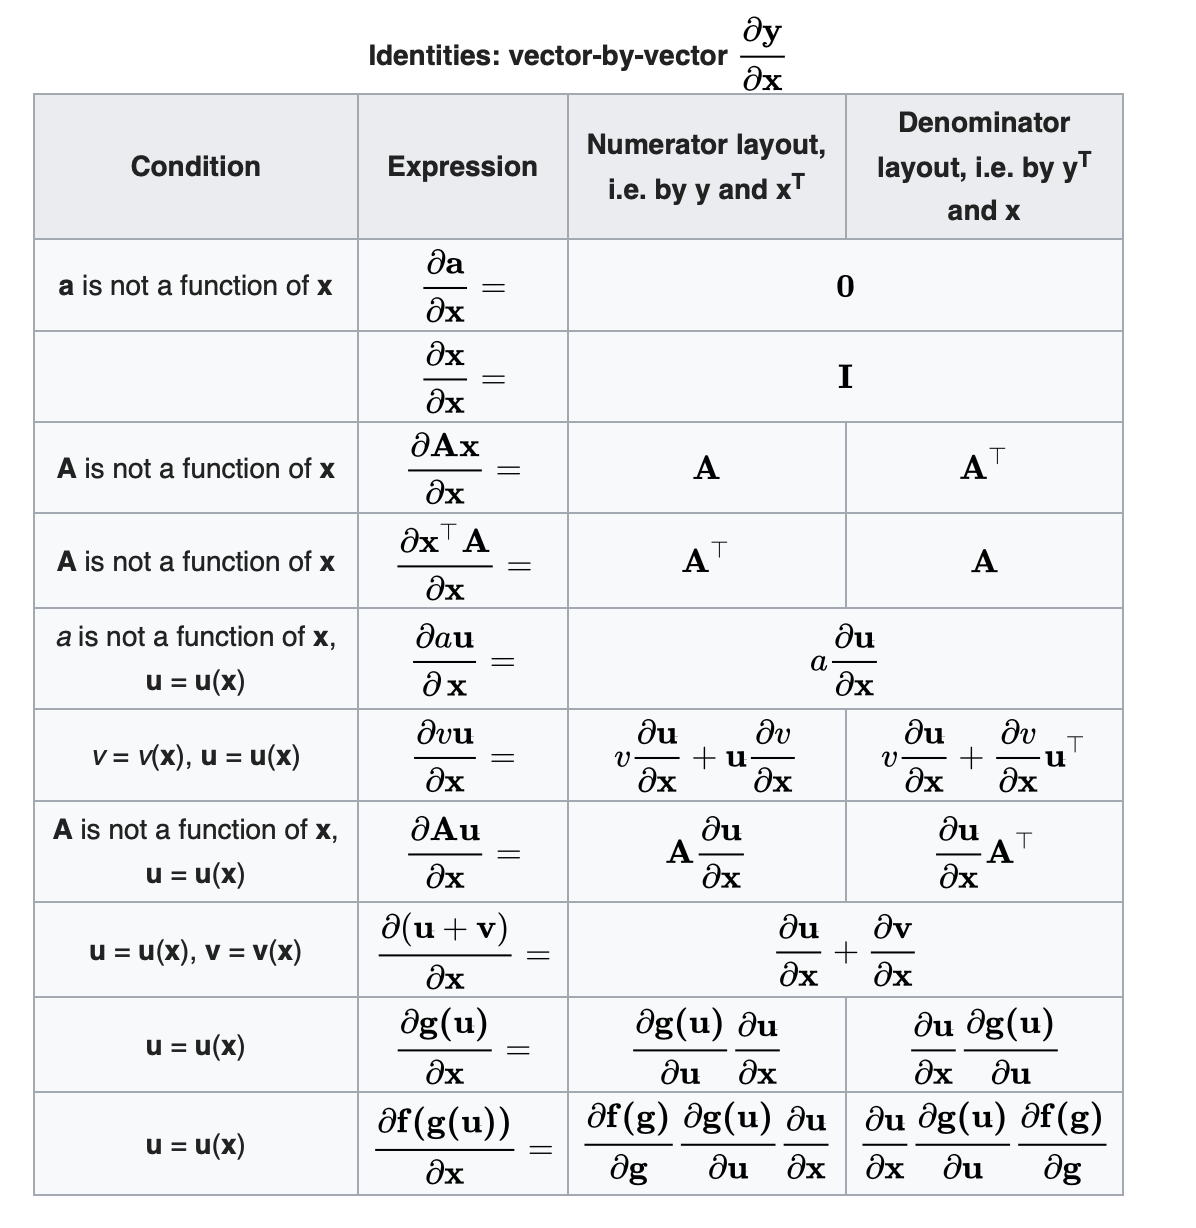
\includegraphics[scale=0.25]{vector_by_vector.png}
    \caption{Denominator layout means $x\in\mathbb{R}^{n\times 1}$}
    \label{}
\end{figure}\end{center}

\begin{equation}
    \begin{aligned}
        \frac{\partial u}{\partial x^T}&=(\frac{\partial u^T}{\partial x})^T\\
        \frac{\partial u^Tv}{\partial x}&=\frac{\partial u^T}{\partial x}v+\frac{\partial v^T}{\partial x}u^T\\
        \frac{\partial uv^T}{\partial x}&=\frac{\partial u}{\partial x}v^T+u\frac{\partial v^T}{\partial x}\\
        \frac{\partial x^Tx}{\partial x}&=2x\\
        \frac{\partial x^TAx}{\partial x}&=(A+A^T)x\\
    \end{aligned}
    \nonumber
\end{equation}
where $x,u,v\in \mathbb{R}^{n\times 1}$

$\textbf{Note:}$ $$\frac{d\|Aw-b\|^2}{dw}
=\frac{d(Aw-b)^T(Aw-b)}{dw}
\\=\frac{d(Aw-b)^T}{dw}(Aw-b)+\frac{d(Aw-b)^T}{dw}(Aw-b)
\\=2A(Aw-b)$$

Matrix by vector:
\begin{equation}
    \begin{aligned}
        \frac{\partial AB}{\partial x}&=\frac{\partial A}{\partial x}B+A\frac{\partial B}{\partial x}
    \end{aligned}
    \nonumber
\end{equation}

Matrix by matrix:
\begin{equation}
    \begin{aligned}
        \frac{\partial u^TXv}{\partial X}&=uv^T\\
        \frac{\partial u^TX^TXu}{\partial X}&=2Xuu^T\\
        \frac{\partial [(Xu-v)^T(Xu-v)]}{\partial X}&=2(Xu-v)u^T\\
    \end{aligned}
    \nonumber
\end{equation}

Trace (迹):
\begin{equation}
    \begin{aligned}
        tr(a)&=a\\
        tr(AB)&=tr(BA)\\
        tr(ABC)=&tr(CAB)=tr(BCA)\\
        \frac{\partial tr(AB)}{\partial A}&=B^T\\
        tr(A)&=tr(A^T)\\
        \frac{\partial tr(ABA^TC)}{\partial A}&=CAB+C^TAB^T
    \end{aligned}
    \nonumber
\end{equation}

\subsection{LU Decomposition}
Triangular matrix saves time when computing $Ax=b$.

Let A be a square matrix. An LU factorization refers to the factorization of A, with proper row and/or column orderings or permutations, into two factors – a lower triangular matrix L and an upper triangular matrix U:

${\displaystyle A=LU.}$
In the lower triangular matrix all elements above the diagonal are zero, in the upper triangular matrix, all the elements below the diagonal are zero. For example, for a 3 × 3 matrix A, its LU decomposition looks like this:

$${\displaystyle {\begin{bmatrix}a_{11}&a_{12}&a_{13}\\a_{21}&a_{22}&a_{23}\\a_{31}&a_{32}&a_{33}\end{bmatrix}}={\begin{bmatrix}\ell _{11}&0&0\\\ell _{21}&\ell _{22}&0\\\ell _{31}&\ell _{32}&\ell _{33}\end{bmatrix}}{\begin{bmatrix}u_{11}&u_{12}&u_{13}\\0&u_{22}&u_{23}\\0&0&u_{33}\end{bmatrix}}.}$$

$$A=PLU$$
$P$ is a permutation matrix (used to swap row, only one $1$ in every row). $P$ is orthogonal, so $P^{-1}=P^T$.

Solve $Ax=b$:
\begin{equation}
    \begin{aligned}
        Ax&=b\\
        PLUx&=b\\
        \text{Let }y=Ux,&\text{ then solve PLy=b}\\
        Ly&=P^Tb
    \end{aligned}
    \nonumber
\end{equation}
Complexity: $O(n^3)$















\begin{thebibliography}{1}
    \bibitem{Long2015Fully}  MATH 417: Christopher J Leininger  \newblock Introduction to Abstract Algebra (Draft)  2017.
    \bibitem{Long2015Fully} MATH 484
    \bibitem{Long2015Fully} ECE 490
    \bibitem{Long2015Fully} STAT 425
    \bibitem{Long2015Fully} CS/MATH 357
\end{thebibliography}


\end{document}
\bibliography{reference}
\bibliographystyle{unsrt}